\documentclass[a4paper,12pt]{article}
\usepackage{jae}
\usepackage{amsmath, bm, amsfonts}

\title{Spatial models for distance sampling data: recent developments and future directions}
\running{Spatial models for distance sampling}

\author{
David L. Miller$^{1*}$, \and
M. Louise Burt$^{2}$, \and
Eric A. Rexstad$^{2}$, \and 
Len Thomas$^{2}$.}

\affiliations{
\item Department of Natural Resources Science, University of Rhode Island, Kingston, Rhode Island 02881, USA
\item Centre for Research into Ecological and Environmental Modelling,\\ The Observatory, University of St. Andrews, St. Andrews KY16 9LZ, UK
}
\nwords{5104}
\ntables{0}
\nfig{6}
\nref{47}

\corr{\url{dave@ninepointeightone.net}}

\begin{document}

\maketitle

\begin{abstract}
  \noindent 

\begin{enumerate}
	\item Our understanding of a biological population can be greatly enhanced by modelling their distribution in space and as a function of environmental covariates. Such models can be used to investigate the relationships between distribution and environmental covariates as well as reliably estimate abundances and create maps of animal/plant distribution. 
	\item Density surface models consist of a spatial model of the abundance of a biological population which has been corrected for uncertain detection via distance sampling methods. 
	\item We review recent developments in the field and consider the likely directions of future research before focussing on a popular approach based on generalized additive models.  In particular, we consider spatial modelling techniques that may be advantageous to applied ecologists such as quantification of uncertainty in a two-stage model and smoothing in areas with complex boundaries.
	\item The methods discussed are available in an \textsf{R} package developed by the authors (\texttt{dsm}) and are largely implemented in the popular Windows software Distance.
\end{enumerate}
 

\end{abstract}

\noindent \textbf{Keywords:} abundance estimation, Distance software, generalized additive models, line transect sampling, point transect sampling, population density, spatial modelling, wildlife surveys


\newpage

\section*{Introduction}
\label{s:intro}

When surveying biological populations it is increasingly common to record spatially referenced data, for example: coordinates of observations, habitat type, elevation or (if at sea) bathymetry. Spatial models allow for vast databases of spatially-referenced data \citep[e.g. OBIS-SEAMAP,][]{Halpin:2009je} to be harnessed, enabling investigation of interactions between environmental covariates and population densities. Mapping the spatial distribution of a population can be extremely useful, especially when communicating results to non-experts. Recent advances in both methodology and software have made spatial modelling readily available to the non-specialist \citep[e.g.,][]{Wood:2006wz, Rue:2009tw}. Here we use ``spatial model'' to refer to any model that includes any spatially referenced covariates, not only those models that include explicit location terms. This article is concerned with combining spatial modelling techniques with distance sampling \citep{Buckland:2001vm, Buckland:2004ts}. 

Distance sampling extends plot sampling to the case where detection is not certain. Observers move along lines or visit points and record the distance from the line or point to the object of interest ($y$). These distances are used to estimate the \textit{detection function}, $g(y)$ (for example, Fig. \ref{dolphin-df}), by modelling the decrease in detectability with increasing distance from the line or point (conventional distance sampling, CDS). The detection function may also include covariates \citep[multiple covariate distance sampling, MCDS;][]{Marques:2007vm} which affect the scale of the detection function. From the fitted detection function, the average probability of detection can be estimated by integrating out distance. The estimated average probability that an animal is detected given that it is in the area covered by the survey, $\hat{p}_i$, can then be used to estimate abundance as

\begin{equation}
\hat{N} = \frac{A}{a} \sum_{i=1}^{n} \frac{s_i}{\hat{p}_i},
\label{ht-est}
\end{equation}
where $A$ is the area of the study region, $a$ is the area covered by the survey (i.e., the sum of the areas of all of the strips/circles) and the summation takes place over the $n$ observed clusters, each of size $s_i$ (if individuals are observed, $s_i=1 \forall i$) \citep[Chapter 3]{Buckland:2001vm}. Often up to half the observations in a plot sampling data set are discarded to ensure the assumption of certain detection is met. In contrast, distance sampling uses observations that would have been discarded to model detection (although typically some detections are discarded beyond a given \textit{truncation distance} during analysis).

Estimators such as eqn (\ref{ht-est}) rely on the design of the study to ensure that abundance estimates over the whole study area (scaling up from the covered region) are valid. This article focusses on \textit{model-based} inference to extrapolate to a larger study area. Specifically, we consider the use of spatially explicit models to investigate the response of biological populations to biotic and abiotic covariates that vary over the study region. A spatially-explicit model can explain the between-transect variation (which is often a large component of the variance in design-based estimates) and so using a model-based approach can lead to smaller variance in estimates of abundance than design-based estimates. Model-based inference also enables the use of data from opportunistic surveys, for example, incidental data arising from ``ecotourism'' cruises \citep{Williams:2006tz}. 

Our aims in creating a spatial model of a biological population are usually two-fold: (i) estimating overall abundance and (ii) investigating the relationship between abundance and environmental covariates. As with any predictions that are outside the range of the data, one should heed the usual warnings regarding extrapolation. For example, if a model contains elevation as a covariate, predictions at high, unsampled elevations are unlikely to be reliable. Frequently, maps of abundance or density are required and any spurious predictions can be visually assessed, as well as by plotting a histogram of the predicted values. A sensible definition of the region of interest avoids prediction outside the range of the data.

In this article we review the current state of spatial modelling of detection-corrected count data, illustrating some recent developments useful to applied ecologists. The methods discussed have been available in Distance software \citep{Thomas:2010cf} for some time but the recent advances covered here have been implemented in a new \textsf{R} package, \texttt{dsm} \citep{Miller:2013to}  and are to be incorporated into Distance.

Throughout this article a motivating data set is used to illustrate the methods. These data are sightings of pantropical spotted dolphins (\textit{Stenella attenuata}) during April and May of 1996 in the Gulf of Mexico.  Observers aboard the NOAA vessel Oregon II recorded sightings and environmental covariates (see \mbox{\url{http://seamap.env.duke.edu/dataset/25}} for survey details). A complete example analysis is provided in Appendix A. The data used in the analysis are available in the \texttt{dsm} package and Distance.

The rest of the article reviews approaches for the spatial modelling of distance sampling data before focussing on the density surface modelling approach of \cite{Hedley:2004et} to estimate abundance and uncertainty. We then describe recent advances and provide practical advice regarding model fitting, formulation and checking. Finally we discuss future directions for research in spatially modelling detection-corrected count data.


\section*{Approaches to spatial modelling of distance sampling data}
\label{s:approaches}

Modelling of spatially referenced distance sampling data is equivalent to modelling spatially-referenced count data, with the additional information provided by collecting distances to account for imperfect detection. We review recent efforts to model such data; some consist of two steps (correction for imperfect detection, then spatial modelling), while others jointly estimate the relevant parameters.

\subsection*{Two-stage approaches}

The focus of this article is the ``count model'' of \cite{Hedley:2004et}, we will henceforth refer to this approach as \textit{density surface modelling} (DSM). Modelling proceeds in two steps: a detection function is fitted to the distance data to obtain detection probabilities for clusters (flocks, pods, etc.) or individuals. Counts are then summarised per segment (contiguous transect section). A generalised additive model \cite[GAM; e.g.][]{Wood:2006wz} is then constructed with the per-segment counts as the response with either counts or segment areas corrected for detectability (see \textit{Density surface modelling}, below). GAMs provide a flexible class of models that include generalized linear models \citep[GLMs;][]{McCullagh:1989ux} but extend them with the possible addition of splines to create smooth functions of covariates, random effects terms or correlation structures. We cover advances using this approach in \textit{Recent developments}.

As with the DSM approach, \cite{Niemi:2010kx} used a two-step procedure: first fitting a detection function, then using a Bayesian point process to model spatial pattern (fitted using MCMC). Object density was described by an intensity function, which included spatially-referenced covariates. A possible disadvantage of their approach was that the distance function was assumed fixed once its parameters are estimated, and thus uncertainty may not be correctly propagated into final abundance estimates.

\cite{VerHoef:2013ky} also included separate density and detection models for seals in the Bering sea. However, they were able to separate the detection process into three components: (i) incomplete detection on the transect line, (ii) declining detection probability as a function of distance, and (iii) availability bias (as seals could only be observed when hauled out on ice flows).  After correcting counts for uncertain detection, they used a hierarchical, zero-inflated spatial regression model to estimate abundance, propagating variance associated with each stage of modelling into final estimates. The analysis shows that when extra information is available (such as telemetry data for the haul-out process) additional insight can be derived.

We note that there are many approaches to modelling spatially referenced count data \citep[][provides an overview of such methods for marine bird modelling]{Oppel:2011tv}. Also worthy of note is the approach of \cite{Barry:2002bm} who used a two-stage approach to model presence/absence then spatial distribution (each via a separate GAM) to account for zero-inflation.

\subsection*{One-stage approaches}

Rather than fitting two separate models, some authors have estimated parameters of the detection and spatial models simultaneously. Perhaps the first such example was \cite{Royle:2004tu}, who considered an integrated likelihood model for point and line transects. The approach views abundance as a nuisance variable which was integrated out of the likelihood, but inferences may still be made about factors affecting underlying density (including covariate effects). This approach was originally developed for binned distance data, but was extended by \cite{Chelgren:2011us} for continuous distance data.

Both \cite{Schmidt:2011ec} and \cite{Conn:2012bx} took data augmentation approaches to add unobserved clusters within their hierarchical Bayesian models. \cite{Schmidt:2011ec} used a presence/absence-type model and a super-population approach \citep[as in][]{Royle:2008wc}. \cite{Conn:2012bx} augmented observations only within the sampled transects using RJMCMC. Looking at the problem with at a coarser spatial resolution (stratum-level), \cite{Moore:2011jf} separated the problem into observation and process components using a state-space model. The process component described the underlying population density as it changed over time and space, which was linked to the data via the detection function. 

Another point process-based approach is that of \cite{Johnson:2010gf}, who used a Poisson process to model the locations of individuals in the survey area. Unlike \cite{Niemi:2010kx}, parameters of the intensity function were estimated jointly with detection function parameters via standard maximum likelihood methods for point processes \citep{Baddeley:2000to} (allowing uncertainty from both the spatial pattern and detection function to be included in variance estimates). A post-hoc correction factor was used to address overdispersion unmodelled by spatial covariates (i.e. counts that do not follow a Poisson mean-variance relationship).

\subsection*{One- vs. two-stage approaches}

Generally very little information is lost by taking a two-stage approach. This is because transects are typically very narrow compared with the width of the study area so, provided no significant density variation takes place ``across'' the width of the lines or within the point, there is no information in the distances about the spatial distribution of animals (this is an assumption of two-stage approaches). 

Two-stage approaches are effectively ``divide and conquer'' techniques: concentrating on the detection function first, and then, given the detection function, fitting the spatial model. One-stage models are more difficult to both estimate and check as both steps occur at once; models are potentially simpler from the perspective of the user and perhaps more mathematically elegant.

 Two-stage models have the disadvantage that to accurately quantify model uncertainty one must appropriately combine uncertainty from the detection function and spatial models. This can be challenging; however, the alternative of ignoring uncertainty from the detection process \cite[e.g.][]{Niemi:2010kx} can produce confidence or credible intervals for abundance estimates that have coverage below the nominal level. More information regarding how variance estimation is addressed for DSMs is given in \textit{Recent developments}.

\section*{Density surface modelling}
\label{s:dsm}

This section focuses on modelling the density/abundance estimation stage of the DSM approach introduced previously. Both line and point transects can be used, but if lines are used then they are are split into contiguous \textit{segments} (indexed by $j$), which are of length $l_j$. Segments should be small enough such that neither density of objects nor covariate values vary appreciably within a segment (making the segments approximately square is usually sufficient; $2w\times 2w$, where $w$ is the truncation distance). The area of each segment enters the model as (or as part of) an offset: the area of segment $j$ is $A_j = 2wl_j$ and for point $j$ is $A_j=\pi w^2$. 

Count or estimated abundance (per  segment or point) is then modelled as a sum of smooth functions of covariates ($z_{jk}$ with $k$ indexing the covariates, e.g., location, sea surface temperature, weather conditions; measured at the segment/point level) using a generalized additive model. Smooth functions are modelled as splines, providing flexible unidimensional (and higher-dimensional) curves (and surfaces, etc) that describe the relationship between the covariates and response. \cite{Wood:2006wz} and \cite{ruppert2003semiparametric} provide more in-depth introductions to smoothing and generalized additive models.

We begin by describing a formulation where only covariates measured per-segment (e.g. habitat, Beaufort sea state) are included in the detection function. We later expand this simple formulation to include observation level covariates (e.g., cluster size, species)

\subsection*{Count as response}

The model for the count per segment is:

\begin{equation*}
\mathbb{E}(n_j) = \hat{p}_j A_j \exp\left[ \beta_0 + \sum_k f_k\left(z_{jk}\right) \right],
\end{equation*}
where the $f_k$s are smooth functions of the covariates and $\beta_0$ is an intercept term. Multiplying the segment area ($A_j$) by the probability of detection ($\hat{p}_j$) gives the \textit{effective area} for segment $j$. If there are no covariates other than distance in the detection function then the probability of detection is constant for all segments (i.e., $\hat{p}_j=\hat{p}$, $\forall j$). The distribution of $n_j$ can be modelled as an overdispersed Poisson, negative binomial, or Tweedie distribution (see \textit{Recent developments}).

Fig. \ref{dolphin-eda} shows the raw observations of the dolphin data, along with the transect lines, overlaid on the depth data. A half-normal detection function was fitted to the distances and is shown in Fig. \ref{dolphin-df}. Fig. \ref{fits-depth} shows a DSM fitted to the dolphin data. The top panel shows predictions from a model where depth was the only covariate, the bottom panel shows predictions where a (bivariate) smooth of spatial location was also included. Comparing the models using GCV score, the latter had a considerably lower score (39.12 vs 48.46) and so would be selected as our preferred model. 

As well as simply calculating abundance estimates, relationships between covariates and abundance can be illustrated via plots of marginal smooths. The effect of depth on abundance (on the scale of the link function) for the dolphin data can be seen in Fig. \ref{depth-gamplot}. 

An alternative to modelling counts is to use the per-segment/circle abundance using distance sampling estimates as the response. In this case we replace $n_j$ by:

\begin{equation*}
\hat{N}_j = \sum_{r=1}^{R_j} \frac{s_{jr}}{\hat{p}_j},
\end{equation*}
where $R_j$ is the number observations in segment $j$ and $s_{jr}$ is the size of the $r^\text{th}$ cluster in segment $j$ (if the animals occur individually then $s_{jr}=1$, $\forall j,r$). 

The following model is then fitted:

\begin{equation*}
\mathbb{E}(\hat{N}_j) = A_j \exp\left[ \beta_0 + \sum_k f_k\left(\bm{z}_{jk}\right) \right],
\end{equation*}
where $\hat{N}_j$, as with $n_j$, is assumed to follow an overdispersed Poisson, negative binomial, or Tweedie distribution (see \textit{Recent developments}, below). Note that the offset ($A_j$) is now the area of segment/point rather than effective area of the segment/point. Although $\hat{N}_j$ can always be modelled instead of $n_j$, it seems preferable to use $n_j$ when possible, as one is then modelling actual (integer) counts as the response rather than estimates. Note that although $\hat{N}_j$ may take non-integer values, this does not present an estimation problem for the response distributions covered here.

\subsubsection*{DSM with covariates at the observation level}

The above models consider the case where the covariates are measured at the segment/point level. Often covariates ($z_{ij}$, for individual/cluster $i$ and segment/point $j$) are collected on the level of observations; for example sex or cluster size of the observed object or identity of the observer. In this case the probability of detection is a function of the object (individual or cluster) level covariates $\hat{p}(z_i)$. Object level covariates can be incorporated into the model by adopting the following estimator of the per-segment/point abundance:

\begin{equation*}
\hat{N}_j = \sum_{r=1}^{R_j} \frac{s_{jr}}{\hat{p}(z_{rj})}.
\end{equation*}

Density, rather than abundance, can be modelled by excluding the offset and instead dividing the count (or estimated abundance) by the area of the segment/point (and weighting observations by the segment/point areas). We concentrate on abundance here; see \cite{Hedley:2004et} for further details on modelling density.

\subsection*{Prediction}

A DSM can be used to predict abundance over a larger/different area than was originally surveyed. In that case the investigator must create a series of prediction cells over the prediction region. For each cell the covariates included in the DSM must be available; the area of each cell is also required. Having made predictions for each cell, these can be plotted as an abundance map (as in Fig. \ref{fits-depth}) and, by summing over cells, an overall estimate of abundance can be calculated. It is worth noting that using prediction grid cells that are smaller than the resolution of the spatially referenced data has no effect on abundance/density estimates.

\subsection*{Variance estimation}

Estimating the variance of abundances calculated using a DSM is not straightforward: uncertainty from the estimated parameters of the detection function must be incorporated into the spatial model. A second consideration is that in a line transect survey, abundances in adjacent segments are likely to be correlated; failure to account for this spatial autocorrelation will lead to artificially low variance estimates and hence misleadingly narrow confidence intervals.

\cite{Hedley:2004et} describe a method of calculating the variance in the abundance estimates using a parametric bootstrap, resampling from the residuals of the fitted model. The bootstrap procedure is as follows.

Denote the fitted values for the model to be $\hat{\bm{\eta}}$. For $b=1,\ldots,B$ (where $B$ is the number of resamples required).
\begin{enumerate}
	\item Resample (with replacement) the per-segment/point residuals, store the values in $\mathbf{r}_{b}$.
	\item Refit the model but with the response set to $\hat{\bm{\eta}}+\mathbf{r}_{b}$ (where $\hat{\bm{\eta}}$ are the fitted values from the orginal model).
	\item Take the predicted values for the new model and store them.
\end{enumerate}
From the predicted values stored in the last step the variance originating in the spatial part of the model can be calculated. The total variance of the abundance estimate (over the whole region of interest or sub-areas) can then be found by combining the variance estimate from the bootstrap procedure with the variance of the probability of detection from the detection function model using the delta method \citep[which assumes that the two components of the variance are independent;][]{verhoef:2012}.

The above procedure assumes that there is no correlation in space between segments, which are usually contiguous along transects. If many animals are observed in a particular segment then we might expect there to be high numbers in the adjacent segments. A moving block bootstrap \citep[MBB;][Section 8.6]{Efron:1993tv} can account for some of this spatial autocorrelation in the variance estimation. The segments are grouped together into overlapping blocks (so if the block size is 5, block one is segments $1,\ldots,5$, block two is segments $2,\ldots,6$, and so on). Then, at step (2) above, resamples are taken at the block level (rather than individual segments within a transect). Using MMB will account for correlation between the segments at scales smaller than the block size, inflating the variances accordingly. Block size can be selected by plotting an autocorrelogram of the residuals from the DSM.

Both bootstrap procedures can also be modified to take detection function uncertainty into account. Distances are simulated from the fitted detection function and then the offset is re-calculated by fitting a detection function to the simulated distances.
 
Uncertainty can be estimated for a given prediction region by calculating the appropriate quantiles of the resulting abundance estimates (outlier removal may be required before quantile calculation). DSM uncertainty can be visualised via a plot of per-cell coefficient of variation obtained by dividing the standard error for each cell by its predicted abundance (as in Fig. \ref{cv-plot}). 

\section*{Recent developments}
\label{s:recentadvances}

\subsubsection*{GAM uncertainty and variance propagation}

Rather than using a bootstrap, one can use GAM theory to construct uncertainty estimates for DSM abundance estimates. This requires that we use the distribution of the parameters in the GAM to simulate model coefficients, using them to generate replicate abundance estimates \citep[further information can found in][page 245]{Wood:2006wz}. Such an approach removes the need to refit the model many times, making variance estimation much faster.
 
\cite{WILLIAMS:2011in} go a step further and incorporate the uncertainty in the estimation of the detection function into the variance of the spatial model, albeit only when segment level covariates are in the DSM. Their procedure is to fit the density surface model with an additional random effect term that characterises the uncertainty in the estimation of the detection function (via the derivatives of the probability of detection, $\hat{p}$, with respect to their parameters). Variance estimates of the abundance calculated using standard GAM theory will include uncertainty from the estimation of the detection function. A more complete mathematical explanation of this result is given in Appendix B.

We consider that propagating the uncertainty in this manner to be preferable to the MBB because it is more computationally efficient meaning investigators can easily and quickly estimate variances of complex models. The confidence intervals produced via variance propagation appear comparable (if not narrower) than their bootstrap equivalents, while maintaining good coverage (results of a small simulation study are given in Appendix C).

Fig. \ref{cv-plot} shows a map of the coefficient of variation for the model which includes both location and depth covariates. Variance has been calculated using the variance propagation method. 

\subsection*{Edge effects}
\label{s:leakage}

Previous work \citep{Ramsay:2002uo,Wang:2007tf,Wood:2008vo,ScottHayward:2011tc,Miller:2012tm} has highlighted the need to take care when smoothing over areas with complicated boundaries, e.g., those with rivers, peninsulae or islands. If two parts of the study area (either side of a river or inlet, say) are inappropriately linked by the model (i.e. if the distance between the points is measured as a straight line, rather than taking into account obstacles) then the boundary feature (river, etc) can be ``smoothed across'' so positive abundances are predicted in areas where animals could not possibly occur. Ensuring that a realistic spatial model has been fitted to the data is essential for valid inference. The soap film smoother of \cite{Wood:2008vo} is an appealing solution: a bivariate smooth function of location that can be included in any GAM but that allows for boundary conditions to be estimated and obeyed for a complex study area. Such an approach can be helpful when uncertainty is estimated via a bootstrap as edge effects can also cause large, unrealistic predictions which can plague other smoothers \citep{Bravington:2009vo}.

Even if the study area does not have a complicated boundary, edge effects can still be problematic. \cite{Miller:2012wy} notes that some smoothers have plane components that tend to cause the fitted surface to increase unrealistically as predictions are made further away from the locations of survey effort. This problem can be alleviated by the using a different type of smoother (e.g. a generalisation of thin plate regression splines called \textit{Duchon splines}).

\subsection*{Tweedie distribution}
\label{s:Tweedie}

The Tweedie distribution offers a flexible alternative to the quasi-Poisson and negative binomial distributions as a response distribution when modelling count data \citep{Candy:2004tb}. In particular it is useful when there are a high proportion of zeros in the data \cite[][]{Shono:2008ge,Peel:2012jc} and avoids multiple-stage modelling of zero-inflated data \cite[as in][]{Barry:2002bm}.

The distribution has three parameters parameters: a mean, dispersion and a third power parameter, which leads to additional flexibility. The distribution does not change appreciably when the power parameter is changed by less than $0.1$ and therefore a simple line search over the possible values for the power parameter is usually a reasonable approach to estimating the parameter. Mark Bravington (pers. comm.) suggested plotting the square root of the absolute value of the residuals against fitted values; a ``flatter'' plot (points forming a horizontal line) give an indication of a ``good'' value. We additionally suggest using the metrics described in the next section for model selection.

Appendix D gives further details about the Tweedie distribution (including its probability density function and further references).

\section*{Practical advice}
\label{s:practical}

A flow diagram of the modelling process for creating a DSM is shown in Fig. \ref{flow}. The diagram shows which methods are compatible with each other and what the options are for modelling a particular data set.

In our experience, it is sensible to obtain a detection function that fits the data as well as possible and only begin spatial modelling after a satisfactory detection function has been obtained. Model selection for the detection function can be performed using AIC and model checking using goodness-of-fit tests given in \citet[Section 11.11]{burnham:2004vd}.  If animals occur in clusters rather than individually, bias can be incurred due to the higher visibility of larger clusters. It may then be necessary to include size as a covariate in the detection function \citep[see][Section 4.8.2.4]{Buckland:2001vm}. For some species cluster size may change according to location, \cite{Ferguson:2006ex} use two GAMs (one to model observed clusters and one to model the cluster size) to deal with spatially-varying cluster size amongst delphinids, though the authors do not present the variance of the resulting predictions.

Smooth terms can be selected using (approximate) $p$-values \cite[][Section 4.8.5]{Wood:2006wz}. An additional useful technique for covariate selection is to use an extra penalty for each term in the GAM allowing smooth terms to be removed from the model during fitting \citep[illustrated in Appendix A;][]{Wood:ub}. Smoothness selection is performed by generalized cross validation (GCV) score, unbiased risk estimator (UBRE) or restricted maximum likelihood (REML) score. When model covariates are effectively functions of one another (e.g. depth could be written as a function of location) GCV and UBRE can suffer from optimisation problems \cite[][Section 4.5.3]{Wood:2006wz} which can lead to unstable models \citep[][]{Wood:ub}. REML provides a fitting criteria with a more pronounced optima which avoids some problems with parameter estimation, though caution should always be taken when dealing with highly correlated covariates. A significant drawback of REML is that scores cannot be used to compare models with different linear terms or offsets \cite[][]{Wood:ub}, though the $p$-value and additional penalty techniques described above can be used to select model terms. We highly recommend the use of standard GAM diagnostic plots; \cite{Wood:2006wz} provides further practical information on GAM model selection and fitting.

In the analysis of the dolphin data we included a smooth of location that nearly doubles the percentage deviance explained (27.3\% to 52.7\%). One can see this when comparing the two plots in Fig. \ref{fits-depth} and the plot of the depth (Fig. \ref{dolphin-eda}), the plot of the model containing only a smooth of depth looks very similar to the raw plot of the depth data. Using a smooth of location can be a primitive way to account for spatial autocorrelation and/or as a proxy for other spatially varying covariates that are unavailable. 

A more sophisticated way to account for spatial autocorrelation between segments (within transects) is to use an autocorrelation structure within the DSM (e.g. autoregressive models). Appendix A shows an example using generalized additive mixed model \cite[GAMMs;][Section 6.6, see Appendix A for an example]{Wood:2006wz} to construct an autoregressive (lag 1) correlation structure. This gives a significant reduction in variance, tightening the confidence interval around the abundance estimate.

In the analysis presented here, spatial location has been transformed from latitude and longitude to kilometres north and east of the centre of the survey region at $(27.01^\circ, -88.3^\circ)$. This is because the bivariate smoother used \citep[the thin plate spline;][]{Wood:2003tc} is isotropic: there is only one parameter controlling the smoothness in both directions. Moving one degree in latitude is not the same as moving one degree in longitude and so using kilometres from the centre of the study region makes the covariates isotropic. Using metric units rather than non-standard units of measure such as degrees or feet throughout makes analysis much easier.

A smooth of an environment-level covariate such as depth can be very useful for assessing the relationships between abundance and the covariate (as in Fig. \ref{depth-gamplot}). Caution should be employed when interpreting smooth relationships and abundance estimates, especially if there are gaps over the range of covariate values. Large counts may occur at large values of depth but if no further observations occur at such a large value, then investigators should be skeptical of any relationship.



\section*{Discussion}
\label{s:discussion}

The use of model-based inference for determining abundance and spatial distribution from distance sampling data presents new opportunities in the field of population assessment. Spatial models can be particularly useful when it comes to prediction: making predictions for some subset of the study area relies on stratification in design-based methods and as such can be rather limited. Our models also allow inference from a sample of sightings to a population in a study area without depending upon a random sample design, and therefore data collected from "platforms of opportunity" \citep{Williams:2006tz} can be used (although a well designed survey is always preferable).

Unbiased estimates are dependent upon either (i) distribution of sampling effort being random throughout the study area (for design-based inference) or (ii) model correctness (for model-based inference).  It is easier to have confidence in the former rather than in the latter because our models are always wrong. Nevertheless model-based inference will play an increasing role in population assessment as the availability of spatially-referenced data increases.

The field is quickly evolving to allow modelling of more complex data building on the basic ideas of density surface modelling. We expect to see large advances in temporal inferences and the handling of zero-inflated data and spatial correlation. These should become more mainstream as modern spatio-temporal modelling techniques are adopted. \cite{Petersen:2011vy} provided a very basic framework for temporal modelling; their model included ``before'' and ``after'' smooth terms to quantify the impact of the construction of an offshore windfarm. Zero-inflation in count data may be problematic and two-stage approaches such as \cite{Barry:2002bm} as well as more flexible response distributions made possible by \cite{Rigby:2005wb} have yet to be exploited by those using distance sampling data. Spatial autocorrelation can be accounted for via approaches that explicitly introduce correlations such as generalized estimating equations \cite[GEEs;][]{Hardin:2003uf} or generalized additive mixed models or via mechanisms such as that of \cite{Skaug:2006gs}, which allow observations to cluster according to one of several states (such as high vs low density patches, possibly in response to temporary agglomerations of prey, although the mechanism is unimportant). These advances should assist both modellers and wildlife managers to make optimal conservation decisions. 

Advances in Bayesian computation \cite[INLA;][]{Rue:2009tw}, make one-step, Bayesian, density surface models computationally feasible (as INLA is an alternative to MCMC). An important step toward such models will be incorporation of detection function estimation into the spatial model. We anticipate that such a direct modelling technique will dominate future developments in the field.

Density surface modelling allows wildlife managers to make best use of the available spatial data to understand patterns of abundance, and hence make better conservation decisions (e.g., about reserve or development placement). The recent advances mentioned here increase the reliability of the outputs from a modelling exercise, and hence the efficacy of these decisions.  Density surface modelling from survey data is an active area of research, and we look forward to further improvements and extensions in the near future.

\section*{Acknowledgments}

We wish to thank Paul Conn, another anonymous reviewer, and the associate editor for their helpful comments. DLM wishes to thank Mark Bravington and Sharon Hedley for their detailed discussions and for providing code for their variance propagation method. Funding for the implementation of the recent advances into the \texttt{dsm} package and Distance software came from the US Navy, Chief of Naval Operations (Code N45), grant number \mbox{N00244-10-1-0057}.

\newpage

\bibliography{dsm-refs}


\newpage


\newpage


\section*{Figures}

\begin{figure}[h!]
  \caption{Estimated detection function for pantropical dolphin clusters overlaid onto the scaled histogram of observed distances. Distances are recorded in metres.}
  \label{dolphin-df}
  \begin{center}
    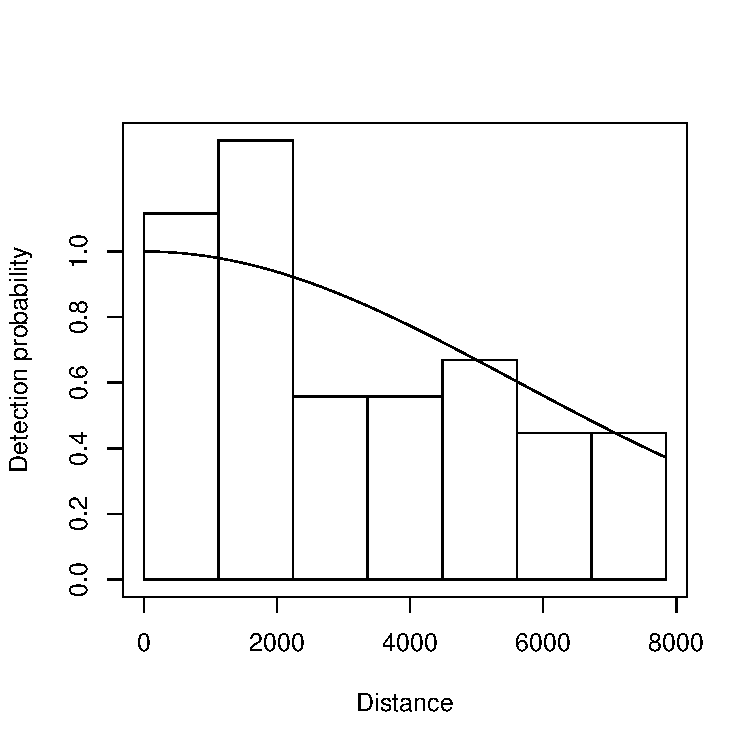
\includegraphics[width=\textwidth]{distances}
  \end{center}
\end{figure}

\newpage

\begin{figure}[h!]
  \caption{The region, transect centrelines and location of detected pantropical dolphin clusters, where size of circle corresponds to the cluster size, overlaid onto depth data.}
  \label{dolphin-eda}
  \begin{center}
    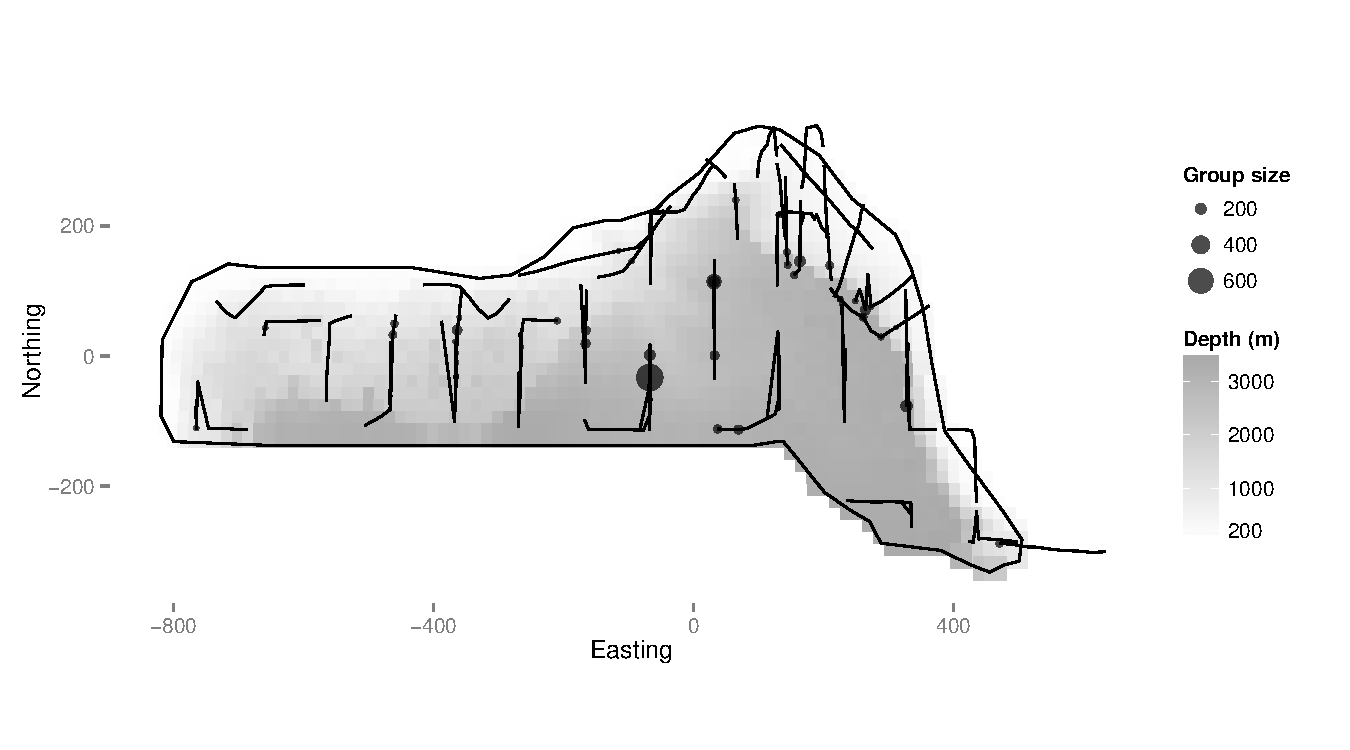
\includegraphics[width=\textwidth]{depth-transects}
  \end{center}
\end{figure}

\newpage

\begin{figure}[h!]
  \caption{Predicted abundance of dolphins from the DSM using only depth as an explanatory variable (top) and the model using both depth and location (bottom).}
  \label{fits-depth}
  \begin{center}
    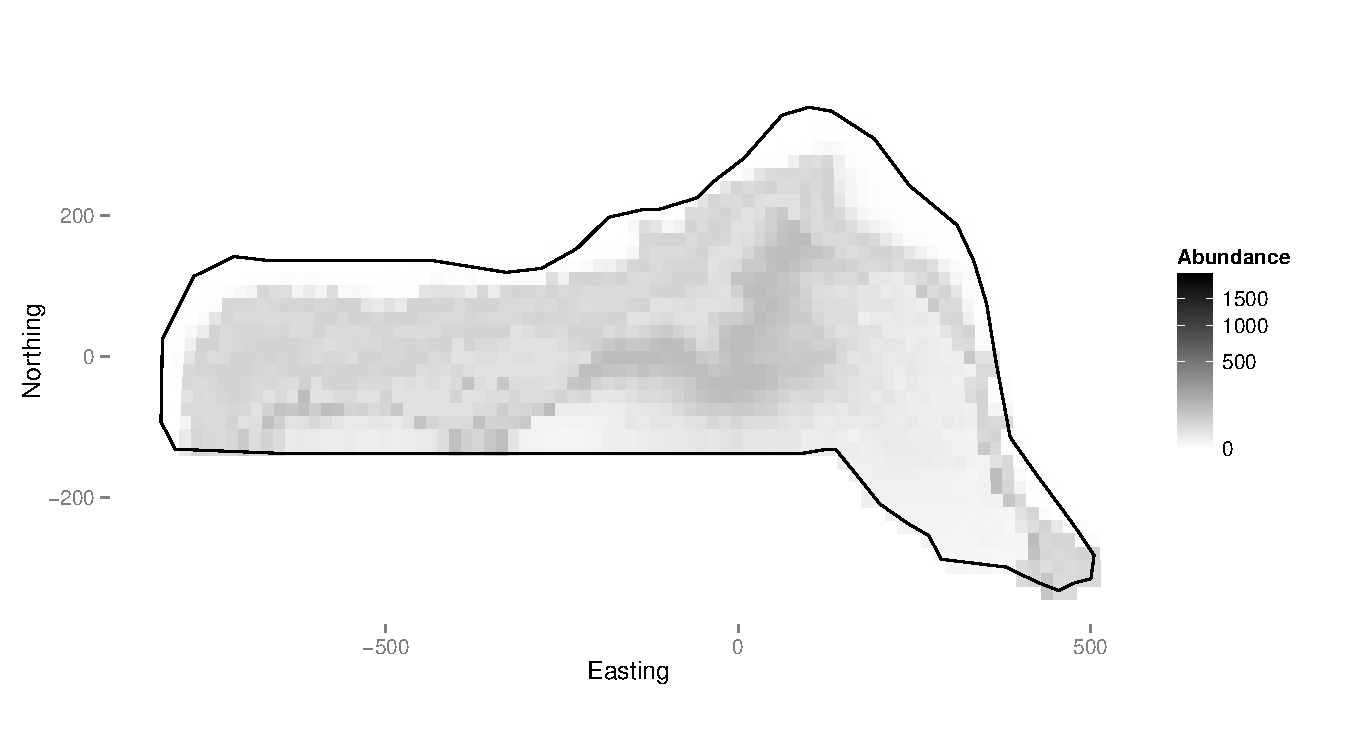
\includegraphics[width=\textwidth]{fit-depth}\\
    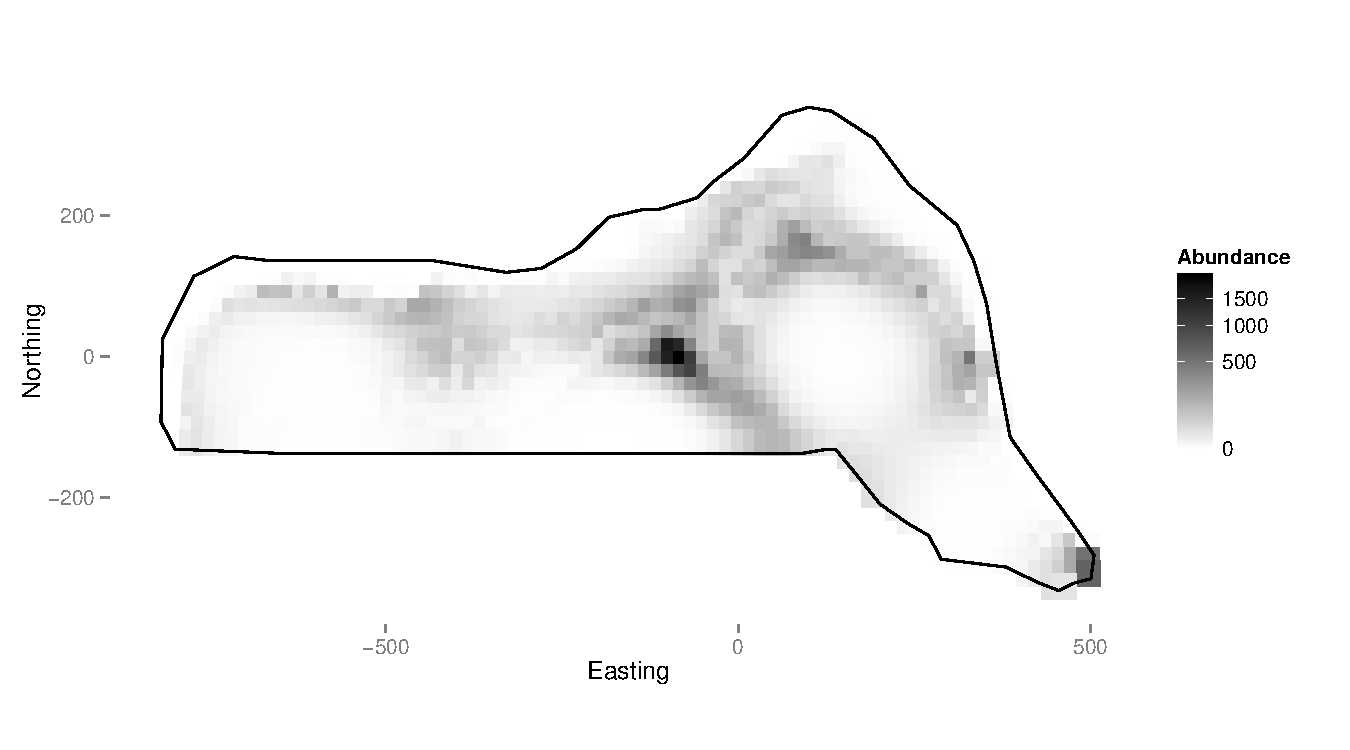
\includegraphics[width=\textwidth]{fit-depth-xy}
  \end{center}
\end{figure}

\newpage

\begin{figure}[h!]
  \caption{Plot of the effect on the response of depth, given location (from the model with both depth and location smooths). Note that it is possible to draw a straight line between 750m and 3000m within the confidence band (between the dashed lines), so the wiggles in the smooth may not be indicative of any relationship. What is clear is that there the estimated number of dolphins increases up to a water depth of about 500m. The rug ticks at the bottom of the plot indicate we have good coverage of the range of depth values in the survey area. Note that the $y$ axis in such plots is on the scale of the link function ($\log$ in this case), so care should be taken in their interpretation.}
  \label{depth-gamplot}
  \begin{center}
    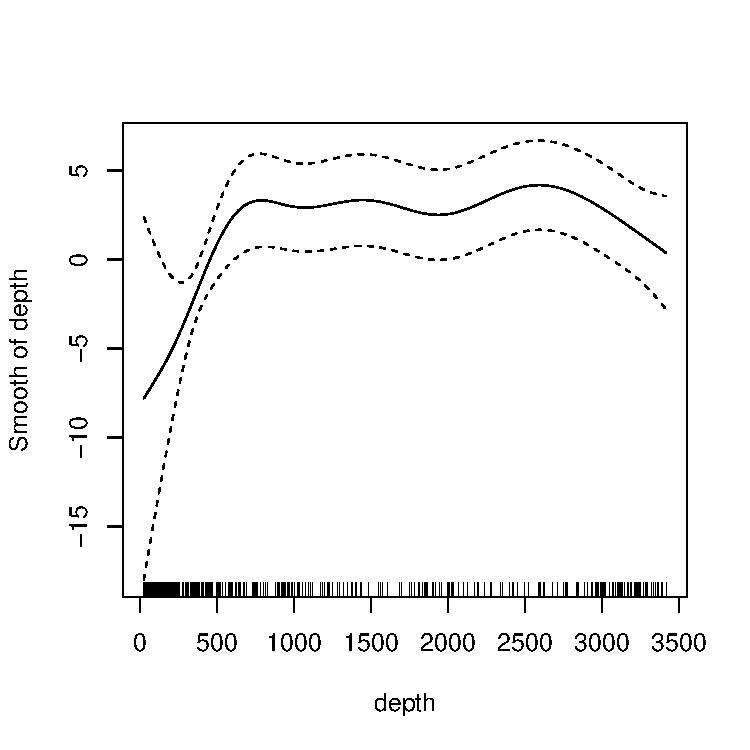
\includegraphics[width=\textwidth]{fit-depth-gam}
  \end{center}
\end{figure}

\newpage

\begin{figure}[h!]
  \caption{Map of the coefficients of variation for the model with smooths of both depth and location. Uncertainty was estimated using the variance propagation method of \cite{WILLIAMS:2011in}. As might be expected, there is high uncertainty where there is low sampling effort (Fig. \ref{dolphin-eda}).}
  \label{cv-plot}
  \begin{center}
    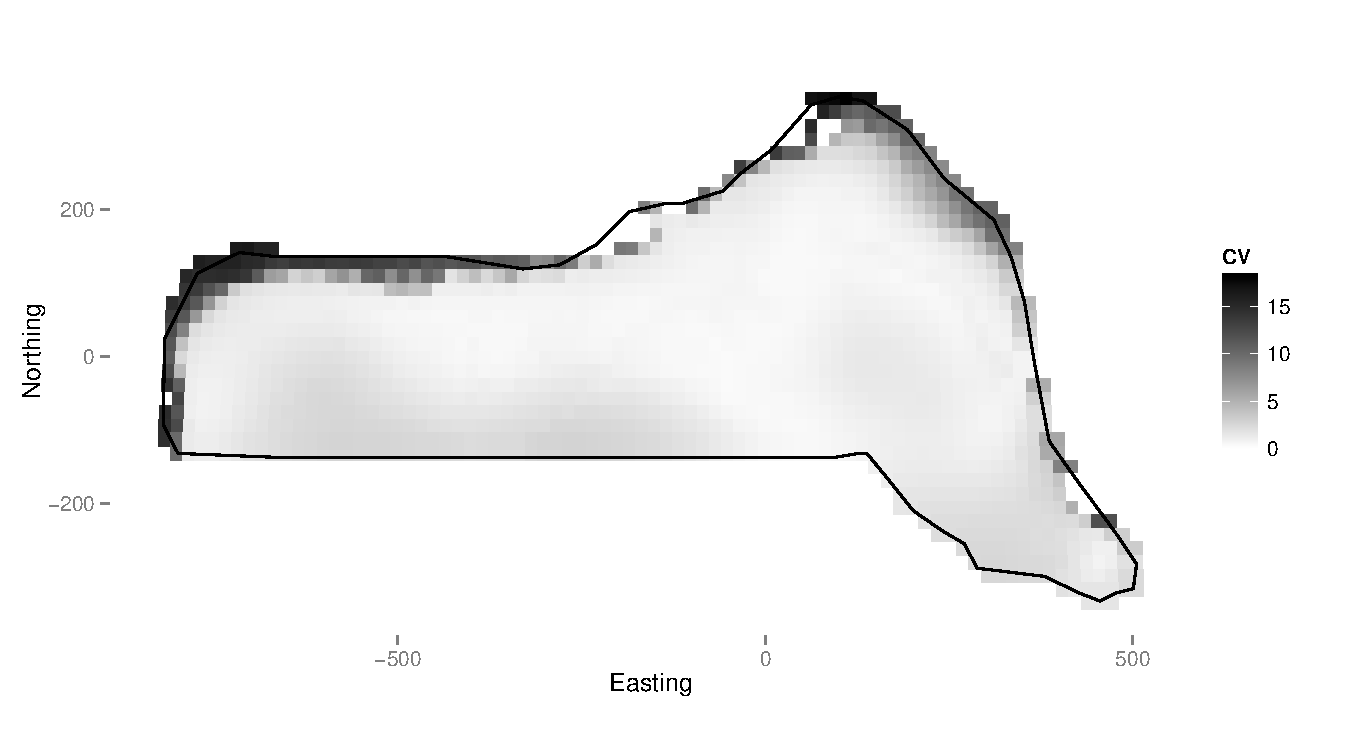
\includegraphics[width=\textwidth]{cvplot-varprop}
  \end{center}
\end{figure}

\newpage

\begin{figure}[h!]
  \caption{Flow diagram showing the modelling process for creating a density surface model.}
  \label{flow}
  \begin{center}
    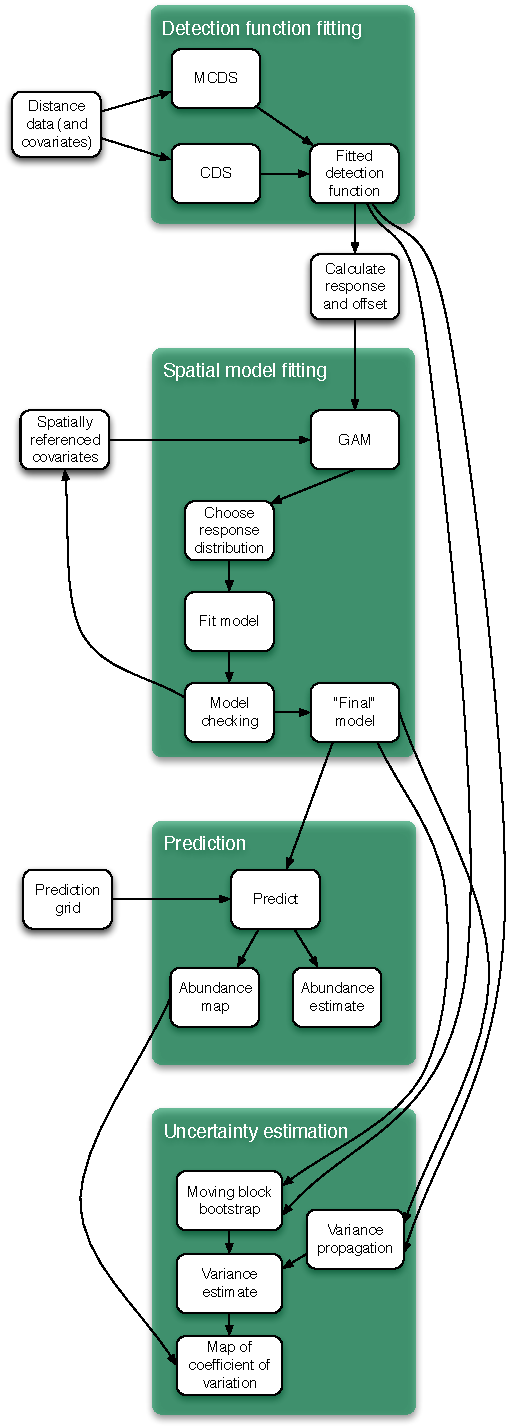
\includegraphics[height=\textheight]{flowdiagram-reduced}
  \end{center}
\end{figure}

\newpage

%\begin{figure}[h!]
%  \caption{Example of model diagnostics for the model which included both location and depth covariates for the dolphin data when a quasi-Poisson response distribution was specified. From top left clockwise:  1) normal Q-Q plot showing a problematic fit (the ``elbow'' in the points), 2) plot of (deviance) residuals against predicted values highlighting outliers and LOESS smooth (\cite{Cleveland:1979vd}) through the point overlaid, 3) a smooth of location fitted to the residuals showing some pattern left in the data and 4) the autocorrelogram. }
%  \label{dsm-check}
%  \begin{center}
%    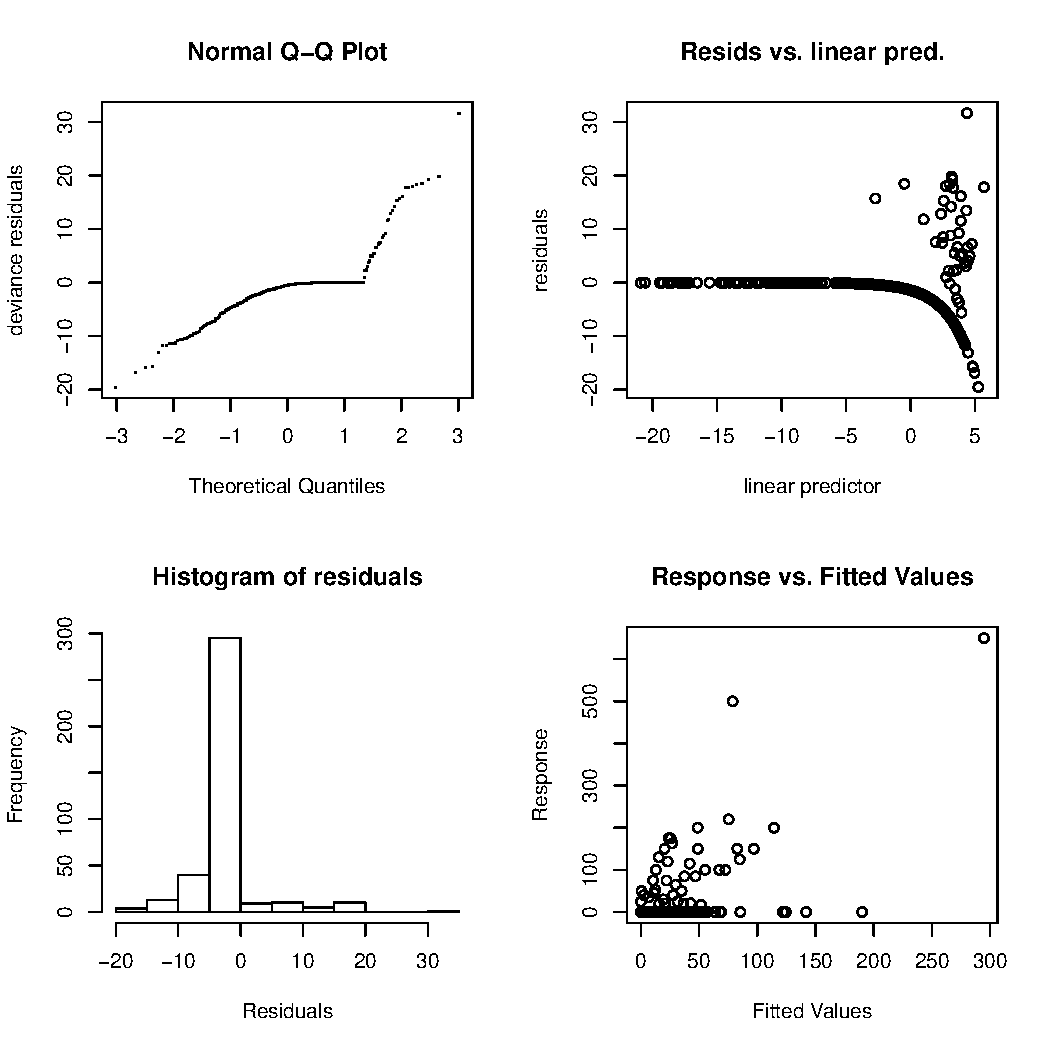
\includegraphics[width=\textwidth]{dsm-check}
%  \end{center}
%\end{figure}


\end{document}
